\section{The guide field}\label{sec:2.2}
The guide field is taken to be static, so the motion of an electron is determined only by the magnetic field strength $\vec{B}$ at each point of its trajectory. As the ideal orbit has been taken to be always horizontal, the field must be purely vertical everywhere on that orbit. I shall make here a further assumption: that the design magnetic field is ideally symmetric with respect to the plane of the ideal orbit.
Taking into account all of the assumptions so far delineated, the magnetic guide field may be characterized completely by giving just two quantities for each azimuthal position $s$, namely, $B_0(s)$, the magnitude of the magnetic field on the ideal orbit, and $(\partial B/\partial x)_{0s}$ the horizontal gradient of the field strength evaluated at the ideal orbit -- that is, at $x = 0$ -- for each azimuth. (Since the field is symmetric with respect to the plane of the ideal orbit $\vec{B}_0$ and $\partial B/\partial x$ have only vertical components, and we need give only their magnitudes). As already mentioned, the field $B_0(s)$ produces the curvature of the ideal orbit; whereas the field gradient $dB/dx$ gives rise to the focussing forces responsible for the stable trajectories near that orbit. The two transverse components of the magnetic field acting on an electron at $(s, x, y)$ may now be written as
\begin{align}
	B_y(s,x,y) &= B_0(s) + \left(\frac{\partial B}{\partial x}\right)_{0s} x\label{eq:2.1}\\
	B_x(s,x,y) &= \left(\frac{\partial B}{\partial x}\right)_{0s} y\label{eq:2.2}
\end{align}

The last relation follows from Maxwell’s equations, which give, for fields with the symmetry imposed here, that $\partial B_x/\partial y = \partial B_y/\partial x$. And the linear approximation has, clearly, been evoked to permit dropping of any terms in the higher derivatives of the fields. The field components above are to be used to obtain the Lorentz force in the equations of motion of the electron.

Storage rings are designed to operate over a range of electron energies. This is accomplished  by arranging that all magnetic fields can be varied together -- being scaled in proportion to the desired operating energy. Clearly if the magnetic field on the design orbit is changed everywhere by the same factor the design orbit will again be a possible trajectory of an electron whose momentum is changed by the same factor. Varying all fields together merely changes the energy to be associated with the design orbit. For these reasons, it is convenient to specify the properties of the guide field in a manner which is independent of any selected operating energy, which is easily done by dividing all fields by a factor proportional to associated electron energy. I choose to define the (linear) properties of the guide field by the two functions
\begin{align}\label{eq:2.3}
	G(s) &= \frac{ecB_0(s)}{E_0}\\
	K_1(s) &= \frac{ec}{E_0} \left(\frac{\partial B}{\partial x}\right)_{0s} \label{eq:2.4}
\end{align}
where $E_0$ is the nominal energy, $c$ is the speed of light, and $e$ is the electronic charge.

Notice that these functions have a simple physical significance. We are here interested only in highly relativistic electrons for which $E = cp$; so $G(s)$ is just the inverse of the radius of curvature $\varrho_s$, of electron of the nominal energy at $x = 0$, $y = 0$.
\begin{align}
	G(s) = \frac{1}{\varrho_s}
\end{align}

We may, then, call $G(s)$ the \textit{curvature function}. The function $K_1(s)$ is the rate of change of the inverse radius with radial displacement.

The functions $G(s)$ and $K_1(s)$ may be fairly arbitrary, but must satisfy a few important constraints. First, $G(s)$ must be such that it does indeed define a closed orbit. (We may think that $G$ \textit{defines} the ideal orbit, or alternatively that some arbitrarily specified closed orbit defines $G$ uniquely.) The change $d\theta_0$ in the direction of the tangent to the ideal orbit in an azimuthal interval $ds$ is
\begin{align}
	-d\theta_0 = \frac{ds}{\varrho_s} = G(s)ds
\end{align}
The angle swept out in one revolution must be $2\pi$; so $G(s)$ must satisfy
\begin{align}
	\int\limits_{0}^{L} G(s)ds = 2\pi
\end{align}
Second, both $G(s)$ and $K_1(s)$ are necessarily periodic functions of $s$, because the azimuthal coordinate $s$ is physically cyclic -- returning to the same point on the orbit after one revolution. We must have that
\begin{align}
	\left\{\begin{array}{rcl}
	\ G(s+L) & = & G(s)\\
	K_1(s+L) & = & K_1(s)
	\end{array}\right.
\end{align}
where $L$ is the orbit length. Except for these constraints, $G(s)$ and $K_1(s)$ may have more or less arbitrary variations with $s$.

Although the guide field functions $G$ and $K_1$ may, in principle, be quite general, it is often convenient to simplify the design or the operation of a storage ring by imposing certain restrictions on them. For example, most electron storage rings are designed to have the same orbit radius, say $\varrho_0$, in all bending magnets - and with no bending at all in the intervening “straight sections” of the orbit. Such a guide field is called \textit{isomagnetic}. The word is perhaps slightly misleading. What is intended is that the magnetic field \textit{on} the design orbit has everywhere the same value \textit{except} where it is zero. Then $G(s)$ is a dichotic function, taking on either the value $G_0$ or zero:
\begin{align}\label{eq:2.9}
	G(s) = \left\{\begin{array}{rrrr}
	G_0 = \frac{1}{\varrho_0}, &&  \text{in magnets}\\
	0, && \text{elsewhere}
	\end{array}\right.
\end{align}
A real guide field cannot, of course, ever be ideally isomagnetic, since it is physically impossible to have a discontinuous magnetic field. There must always be a transition zone at the edge of a magnet in which the field goes from zero to its nominal value. The idealized isomagnetic approximation is, however, generally quite adequate for most purposes.

Although accelerators and storage rings are often built with bending magnets which have also radial gradients of the field, it is quite common nowadays to design separated function guide fields in which the focussing functions and bending functions are assigned to different magnetic elements. That is, the guide field consists of a sequence of flat bending magnets (with no gradient) and quadrupoles (with no field on the design orbit). I shall define a separated function guide field as one for which the functions $G(s)$ and $K_1(s)$ are only separately different from zero. So that we have the condition that
\begin{align}
	G(s)K_1(s) = 0\label{eq:2.10}
\end{align}

One note of caution. It is sometimes convenient to design bending magnets whose pole faces are rectangular. With such a magnet, the design orbit must enter or leave the magnet at other than a right angle to the pole edge. (See Fig. \ref{fig:fig8}).Even if the magnet is “flat” (no radial gradient in the magnet) there will be radial gradients at the edges, where the field is not zero. Equation \eqref{eq:2.10} is not satisfied at the edges, and a guide field constructed of such rectangular magnets - together with quadrupoles - would not strictly satisfy my definition of ``separated function'', although they are often referred to as such. Such guide fields may however, still be isomagnetic.

\begin{figure}[!htb]
	\centering
	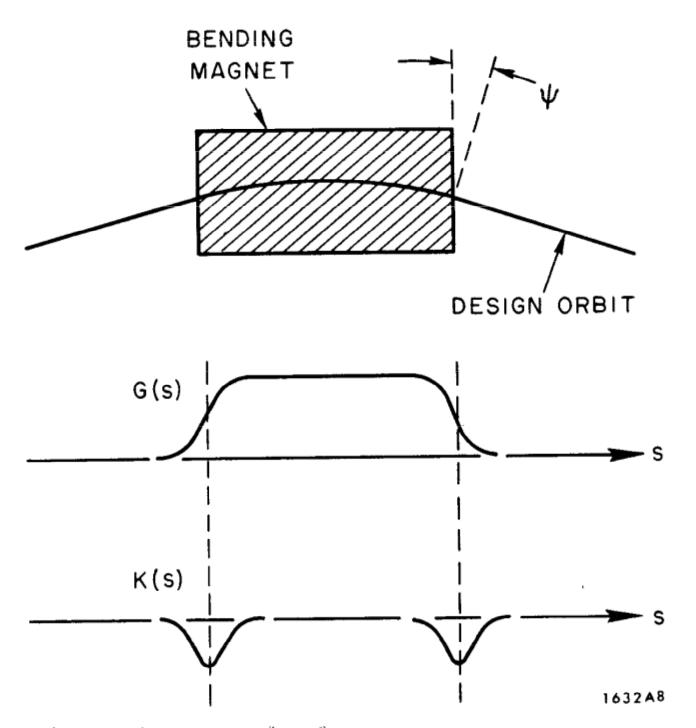
\includegraphics[width=0.6\linewidth]{./Figuras/fig08.jpeg}
	\caption{Guide field with a rectangular magnet.}
	\label{fig:fig8}
\end{figure}
